\documentclass[]{book}
\usepackage{lmodern}
\usepackage{amssymb,amsmath}
\usepackage{ifxetex,ifluatex}
\usepackage{fixltx2e} % provides \textsubscript
\ifnum 0\ifxetex 1\fi\ifluatex 1\fi=0 % if pdftex
  \usepackage[T1]{fontenc}
  \usepackage[utf8]{inputenc}
\else % if luatex or xelatex
  \ifxetex
    \usepackage{mathspec}
  \else
    \usepackage{fontspec}
  \fi
  \defaultfontfeatures{Ligatures=TeX,Scale=MatchLowercase}
  \newcommand{\euro}{€}
\fi
% use upquote if available, for straight quotes in verbatim environments
\IfFileExists{upquote.sty}{\usepackage{upquote}}{}
% use microtype if available
\IfFileExists{microtype.sty}{%
\usepackage{microtype}
\UseMicrotypeSet[protrusion]{basicmath} % disable protrusion for tt fonts
}{}
\usepackage[margin=1in]{geometry}
\usepackage{hyperref}
\PassOptionsToPackage{usenames,dvipsnames}{color} % color is loaded by hyperref
\hypersetup{unicode=true,
            pdftitle={Estudo sobre varas empresariais na Comarca de São Paulo},
            pdfauthor={Associação Brasileira de Jurimetria},
            pdfborder={0 0 0},
            breaklinks=true}
\urlstyle{same}  % don't use monospace font for urls
\usepackage{natbib}
\bibliographystyle{apalike}
\usepackage{color}
\usepackage{fancyvrb}
\newcommand{\VerbBar}{|}
\newcommand{\VERB}{\Verb[commandchars=\\\{\}]}
\DefineVerbatimEnvironment{Highlighting}{Verbatim}{commandchars=\\\{\}}
% Add ',fontsize=\small' for more characters per line
\usepackage{framed}
\definecolor{shadecolor}{RGB}{248,248,248}
\newenvironment{Shaded}{\begin{snugshade}}{\end{snugshade}}
\newcommand{\KeywordTok}[1]{\textcolor[rgb]{0.13,0.29,0.53}{\textbf{{#1}}}}
\newcommand{\DataTypeTok}[1]{\textcolor[rgb]{0.13,0.29,0.53}{{#1}}}
\newcommand{\DecValTok}[1]{\textcolor[rgb]{0.00,0.00,0.81}{{#1}}}
\newcommand{\BaseNTok}[1]{\textcolor[rgb]{0.00,0.00,0.81}{{#1}}}
\newcommand{\FloatTok}[1]{\textcolor[rgb]{0.00,0.00,0.81}{{#1}}}
\newcommand{\ConstantTok}[1]{\textcolor[rgb]{0.00,0.00,0.00}{{#1}}}
\newcommand{\CharTok}[1]{\textcolor[rgb]{0.31,0.60,0.02}{{#1}}}
\newcommand{\SpecialCharTok}[1]{\textcolor[rgb]{0.00,0.00,0.00}{{#1}}}
\newcommand{\StringTok}[1]{\textcolor[rgb]{0.31,0.60,0.02}{{#1}}}
\newcommand{\VerbatimStringTok}[1]{\textcolor[rgb]{0.31,0.60,0.02}{{#1}}}
\newcommand{\SpecialStringTok}[1]{\textcolor[rgb]{0.31,0.60,0.02}{{#1}}}
\newcommand{\ImportTok}[1]{{#1}}
\newcommand{\CommentTok}[1]{\textcolor[rgb]{0.56,0.35,0.01}{\textit{{#1}}}}
\newcommand{\DocumentationTok}[1]{\textcolor[rgb]{0.56,0.35,0.01}{\textbf{\textit{{#1}}}}}
\newcommand{\AnnotationTok}[1]{\textcolor[rgb]{0.56,0.35,0.01}{\textbf{\textit{{#1}}}}}
\newcommand{\CommentVarTok}[1]{\textcolor[rgb]{0.56,0.35,0.01}{\textbf{\textit{{#1}}}}}
\newcommand{\OtherTok}[1]{\textcolor[rgb]{0.56,0.35,0.01}{{#1}}}
\newcommand{\FunctionTok}[1]{\textcolor[rgb]{0.00,0.00,0.00}{{#1}}}
\newcommand{\VariableTok}[1]{\textcolor[rgb]{0.00,0.00,0.00}{{#1}}}
\newcommand{\ControlFlowTok}[1]{\textcolor[rgb]{0.13,0.29,0.53}{\textbf{{#1}}}}
\newcommand{\OperatorTok}[1]{\textcolor[rgb]{0.81,0.36,0.00}{\textbf{{#1}}}}
\newcommand{\BuiltInTok}[1]{{#1}}
\newcommand{\ExtensionTok}[1]{{#1}}
\newcommand{\PreprocessorTok}[1]{\textcolor[rgb]{0.56,0.35,0.01}{\textit{{#1}}}}
\newcommand{\AttributeTok}[1]{\textcolor[rgb]{0.77,0.63,0.00}{{#1}}}
\newcommand{\RegionMarkerTok}[1]{{#1}}
\newcommand{\InformationTok}[1]{\textcolor[rgb]{0.56,0.35,0.01}{\textbf{\textit{{#1}}}}}
\newcommand{\WarningTok}[1]{\textcolor[rgb]{0.56,0.35,0.01}{\textbf{\textit{{#1}}}}}
\newcommand{\AlertTok}[1]{\textcolor[rgb]{0.94,0.16,0.16}{{#1}}}
\newcommand{\ErrorTok}[1]{\textcolor[rgb]{0.64,0.00,0.00}{\textbf{{#1}}}}
\newcommand{\NormalTok}[1]{{#1}}
\usepackage{longtable,booktabs}
\usepackage{graphicx,grffile}
\makeatletter
\def\maxwidth{\ifdim\Gin@nat@width>\linewidth\linewidth\else\Gin@nat@width\fi}
\def\maxheight{\ifdim\Gin@nat@height>\textheight\textheight\else\Gin@nat@height\fi}
\makeatother
% Scale images if necessary, so that they will not overflow the page
% margins by default, and it is still possible to overwrite the defaults
% using explicit options in \includegraphics[width, height, ...]{}
\setkeys{Gin}{width=\maxwidth,height=\maxheight,keepaspectratio}
\setlength{\parindent}{0pt}
\setlength{\parskip}{6pt plus 2pt minus 1pt}
\setlength{\emergencystretch}{3em}  % prevent overfull lines
\providecommand{\tightlist}{%
  \setlength{\itemsep}{0pt}\setlength{\parskip}{0pt}}
\setcounter{secnumdepth}{5}

%%% Use protect on footnotes to avoid problems with footnotes in titles
\let\rmarkdownfootnote\footnote%
\def\footnote{\protect\rmarkdownfootnote}

%%% Change title format to be more compact
\usepackage{titling}

% Create subtitle command for use in maketitle
\newcommand{\subtitle}[1]{
  \posttitle{
    \begin{center}\large#1\end{center}
    }
}

\setlength{\droptitle}{-2em}
  \title{Estudo sobre varas empresariais na Comarca de São Paulo}
  \pretitle{\vspace{\droptitle}\centering\huge}
  \posttitle{\par}
  \author{Associação Brasileira de Jurimetria}
  \preauthor{\centering\large\emph}
  \postauthor{\par}
  \predate{\centering\large\emph}
  \postdate{\par}
  \date{2016-11-28}


% Redefines (sub)paragraphs to behave more like sections
\ifx\paragraph\undefined\else
\let\oldparagraph\paragraph
\renewcommand{\paragraph}[1]{\oldparagraph{#1}\mbox{}}
\fi
\ifx\subparagraph\undefined\else
\let\oldsubparagraph\subparagraph
\renewcommand{\subparagraph}[1]{\oldsubparagraph{#1}\mbox{}}
\fi

\usepackage{booktabs}

\begin{document}
\maketitle

{
\setcounter{tocdepth}{1}
\tableofcontents
}
\chapter{Preâmbulo}\label{preambulo}

Este é um relatório escrito em \textbf{Markdown} descrevendo um estudo
realizado para a corregedoria do Tribunal de Justiça de São Paulo. O
estudo em questão teve a finalidade de auxiliar a tomada de decisão na
criação das varas especializadas em direito comercial na Comarca de São
Paulo.

Para compilar este relatório, você precisará da versão de
desenvolvimento do pacote \textbf{bookdown} disponível no Github do
rstudio:

\begin{Shaded}
\begin{Highlighting}[]
\NormalTok{devtools::}\KeywordTok{install_github}\NormalTok{(}\StringTok{"rstudio/bookdown"}\NormalTok{)}
\end{Highlighting}
\end{Shaded}

Cada arquivo Rmd contém um e apenas um capítulo, e cada capítulo é
definido pelo primeiro nível de cabeçalho \texttt{\#}.

Para compilar este documento em PDF, você precisará utilizar XeLaTeX.

\chapter{Introdução}\label{introducao}

A especialização de varas é um tema de interesse na administração do
judiciário. Atualmente, os poucos estudos disponíveis fazem muitas
suposições para chegar às conclusões ou esbarram em dificuldades
impostas pela documentação dos dados.

Nesse estudo, discutimos a criação de varas empresariais na Comarca de
São Paulo e desenvolvemos metodologias inovadoras para resolver três
problemas. O primeiro é a vinculação de normas para determinação de
competências com assuntos da Tabela Processual Unificada do CNJ (Res.
46). O segundo é o tratamento de falhas na classificação dos assuntos na
base de dados analisada. O terceiro é criar uma métrica de mensuração e
comparação dos esforços empreendidos por magistrados em processos comuns
e empresariais.

Nas análises realizadas, encontramos evidências de que um processo
empresarial demanda aproximadamente o dobro de esforço do que um
processo comum. Ao realizar correções no volume processual a partir de
um modelo de tratamento dos assuntos, concluímos que dois é o número
ideal de varas empresariais que devem ser instaladas para atendimento da
demanda existente.

\section{Objetivo do estudo}\label{objetivo-do-estudo}

O presente estudo tem como objetivo geral fornecer insumos quantitativos
para analisar o tema da especialização de varas empresariais. Por conta
da existência de critérios de criação de varas, que serão explicitados
na sequência, duas atividades receberão maior atenção no decorrer do
relatório, sendo elas

\begin{itemize}
\tightlist
\item
  Estimar o volume de processos empresariais distribuídos por ano nas 45
  varas cíveis do Foro Central.
\item
  Propor uma métrica de esforço do juíz em um processo e comparar o
  esforço médio em processos empresariais contra o esforço médio em
  processos não empresariais.
\end{itemize}

\section{Critérios para criação de
varas}\label{criterios-para-criacao-de-varas}

O Provimento n. 82/2011 do Tribunal de Justiça de São Paulo (TJSP)
dispõe em seu artigo 4º que a criação de novas unidades ou a
especialização das varas existentes obedecerá aos seguintes critérios:

\begin{enumerate}
\def\labelenumi{\arabic{enumi}.}
\tightlist
\item
  a análise levará em conta, preferencialmente, os feitos distribuídos,
  e considerará as características da vara (natureza da jurisdição,
  complexidade da distribuição, entrância em que classificada, etc);
\item
  a distância da sede e a população local, para a criação de foros
  distritais ou regionais. A distância será indicada em quilômetros,
  segundo as vias usuais de acesso;
\item
  a carga de serviço por juiz nas varas antigas e nas varas novas, que
  resultar da instalação, entendido, como número mínimo para deflagrar o
  procedimento de criação, 1.800 processos novos por ano nas varas
  cíveis, de família e da fazenda pública, excluídas as precatórias e as
  execuções fiscais; 600 denúncias por ano, nas varas criminais; e a
  proporção dessas quantidades nas varas cumulativas, conforme a
  representatividade de cada um. A carga de trabalho nos Juizados
  Especiais Cíveis e Criminais será examinada caso a caso, ante a
  especificidade da jurisdição;
\item
  preferencialmente, não haverá redistribuição de feitos, mesmo em caso
  de especialização de varas, prorrogando-se, nesta hipótese, a
  jurisdição das varas em relação aos feitos já distribuídos e com
  observância do Provimento CG- 442/91 (grifos nossos).
\end{enumerate}

Nesse estudo, focamos principalmente no terceiro item. Esta escolha se
justifica pela importância do tópico e a possibilidade de levantamento
de dados quantitativos a partir das bases do Tribunal.

\section{Base de dados}\label{base-de-dados}

Compõe a população em estudo o conjunto de processos distribuídos entre
01/01/2013 e 31/12/2015 em 44 Varas Cíveis e nas 2 varas especializadas
em falência e recuperação judicial do Foro Central Cível da Comarca de
São Paulo.

As seguintes informações foram fornecidas pela Secretaria de Tecnologia
de Informação (STI) do TJSP:

\begin{itemize}
\tightlist
\item
  Número do processo
\item
  Autor
\item
  Réu
\item
  Vara
\item
  Assunto, segundo as categorias descritas na tabela unificada de
  assuntos do Conselho Nacional de Justiça (CNJ).
\item
  Classe, segundo as categorias descritas na tabela unificada de
  assuntos do CNJ.
\item
  Data de distribuição
\item
  Lista de movimentações contendo:

  \begin{itemize}
  \tightlist
  \item
    Data da movimentação
  \item
    Título da movimentação, remotamente inspirado nas categorias
    descritas na tabela unificada de movimentações do CNJ.
  \end{itemize}
\end{itemize}

\chapter{Metodologia}\label{metodologia}

\section{Critérios de identificação de processos
empresariais}\label{criterios-de-identificacao-de-processos-empresariais}

A construção de um critério claro e reprodutível de classificação de
processos empresariais é importante tanto para fins de contagem quanto
para fins de mensuração de esforços. Para executar essa tarefa,
começaremos construindo uma lista de assuntos processuais, campo
disponível no sistema e-SAJ, que estejam relacionados à matéria
empresarial, utilizando como ponto de partida a tabela unificada de
assuntos do CNJ (Res. 46) e a competência das Câmaras Especializadas em
Direito Comercial.

Segundo a Resolução 623/2013 do TJSP, as matérias sob jurisdição das
Câmaras Especializadas em Direito Comercial correspondem ao disposto nos
quatro primeiros itens da lista abaixo. Entretanto, sob orientação da
Corregedoria do TJSP, incluímos dois tópicos extras na nossa lista de
assuntos.

\begin{enumerate}
\def\labelenumi{\arabic{enumi}.}
\tightlist
\item
  Resolução 623/2013

  \begin{enumerate}
  \def\labelenumii{\arabic{enumii}.}
  \tightlist
  \item
    Artigos 966 a 1195 do Livro II do Código Civil (Lei 10.406/02).
  \item
    Lei das Sociedades Anônimas (Lei 9.604/76).
  \item
    Lei da Propriedade Industrial (Lei 9.279/96).
  \item
    Lei das Franquias (Lei 8.955/94).
  \end{enumerate}
\item
  Tópicos adicionais

  \begin{enumerate}
  \def\labelenumii{\arabic{enumii}.}
  \tightlist
  \item
    Procedimentos arbitrais.
  \item
    Artigos 710 a 721 do Código Civil (Lei 10.406/02).
  \end{enumerate}
\end{enumerate}

Após filtrar os assuntos da tabela de assuntos do CNJ associados a esses
dispositivos, obtivemos a lista de assuntos descrita na Tabela
\ref{tab:cnj}.

Se o procedimento adotado consistisse apenas na construção dessa lista,
ele estaria vulnerável a erros de registro, pois alguns processos foram
classificados com assuntos mais genéricos do que os especificados na
Tabela \ref{tab:cnj}. Por isso, a quantidade de processos empresariais
obtida dessa forma subestima a real quantidade de processos
empresariais, se considerarmos que existe uma parcela destes que está
registrada incorretamente. Denominamos por \emph{cifra oculta} a
quantidade não observada de processos empresariais.

Uma forma de contornar esse problema é reclassificar uma parcela ou a
totalidade dos processos com assuntos genéricos como empresariais. Na
nossa aplicação, isso foi feito estimando a probabilidade de um
determinado processo mal classificado ser, na verdade, de matéria
empresarial. Para isso, utilizamos a parcela da base de dados que foi
classificada corretamente e calculamos a proporção de processos
empresariais para cada assunto. A cifra oculta é estimada somando-se as
probabilidades obtidas.

\section{Mensuração do esforço do juiz em cada
processo}\label{metotempos}

Definido um critério para identificação de processos empresariais e
estimação da cifra oculta, o desafio passa a ser o de mensurar
quantitativamente a razão do esforço despendido por um juiz para tratar
de processos empresariais com relação a procedimentos comuns. Essa taxa
é útil pois possibilita a comparação das cargas de trabalho nos dois
regimes.

A mensuração do esforço está ligada ao tema de complexidade processual,
um tópico de pesquisa com muitos eixos de investigação. Até o momento,
não há consenso sobre quais metodologias são mais adequadas em cálculos
dessa natureza, mas NUNES (2016) oferece algumas sugestões tais como a
avaliação do tempo, quantidade de movimentações, quantidade de recursos,
partes e valores envolvidos. É possível definir inclusive o conceito de
\emph{viscosidade processual}:

\begin{quote}
{[}\ldots{}{]} A viscosidade processual pode ser definida como o
conjunto de características estruturais de um processo, capazes de
afetar a sua velocidade. Insistindo na analogia com os fluidos, se um
observador separar dois copos, um cheio de mel e outro de água, e
virá-los simultaneamente de ponta cabeça, a água cairá mais rápido do
que o mel. A maior velocidade da água decorre não da resistência
oferecida por um obstáculo externo ao seu deslocamento, mas de
diferenças na estrutura íntima de cada substância: o mel é viscoso e
avança mais vagarosamente do que a água, que é mais fluida.
\end{quote}

\begin{quote}
Seguindo na analogia, também alguns processos são mais viscosos que ou-
tros. Processos que envolvam matérias complexas, múltiplas partes ou a
produção de provas técnicas elaboradas possuem uma estrutura íntima mais
complexa e tendem a avançar mais lentamente do que casos simples, com
duas partes e que envolvam a produção apenas de prova documental. Essa
complexidade interna é o que chamamos de viscosidade processual, e sua
mensuração é fundamental para administrar a carga de trabalho e as metas
dos funcionários da justiça, como, por exemplo, na criação de regras
para ponderar a distribuição de recursos para as câmaras reservadas.
\end{quote}

Nas análises que seguem, a viscosidade não será utilizada exatamente da
forma como foi definida, mas será o ponto de partida para a
quantificação do volume de trabalho em processos empresariais e comuns.
Como a viscosidade de um fluido está associada à velocidade com que ele
escorre em um determinado meio, no contexto jurídico ela estaria
associada ao tempo de tramitação dos processos.

Para refinar o conceito, propomos a medição da viscosidade através da
medição do tempo decorrido entre atos processuais em dois contextos: i)
o tempo associado à movimentações serventuárias e ii) o tempo associado
à decisões judiciais e outras intervenções dos magistrados. Justificamos
essa separação admitindo que o tempo gasto pelos magistrados em uma
determinada classe de processos fornece uma informação com relação à
complexidade jurídica e factual do procesos que é diferente da
informação fornecida pelo tempo gasto pelo serventuário.

Seguindo essa linha de raciocínio e considerando a finalidade desse
estudo, a criação de varas especializadas, vamos definir viscosidade
processual como o tempo gasto para a tomada de decisão dos magistrados.
Em termos mais precisos, considere \(T_i, \ i = 1,\dots,n\) as datas das
movimentações disponíveis no sistema e-SAJ de um certo processo, sendo
\(n\) o seu número de movimentações. Considere também uma variável
\(D_i, \ i = 1,\dots,n\) que assume valor \(1\) se a \(i\)-ésima
movimentação é uma decisão, um despacho ou uma sentença e \(0\) em caso
contrário. Definimos a viscosidade como

\[ 
V = \sum\limits_{i=2}^n D_i \times (T_i - T_{i-1}), 
\]

\noindent que pode ser simplificada quando consideramos apenas os termos
em que \(D_i > 0\)

\[ 
V = \sum\limits_{\text{decisões}} (T_{\text{decisão}} - T_{\text{última movimentação}})
\]

Um obstáculo para a aplicação da metodologia reside na dificuldade de
decidir se, num determinado processo, o magistrado gastará mais tempo
decidindo ou se todas as suas intervenções já foram realizadas. Para
resolver esse problema, os tempos foram estudados a partir de técnicas
de Análise de Sobrevivência (MILLER; RUPERT, 2011), uma área da
estatística que estuda dados com informações incompletas.

Um exemplo comum desse tipo de análise é o estudo de tempos de falha de
equipamentos (por exemplo, lâmpadas domésticas). Como é inviável
aguardar a quebra de todos equipamentos, no momento da análise temos
indivíduos que falharam (tempo pontual) e indivíduos que falharão no
futuro (censura à direita). A dificuldade disso é que os casos que ainda
não quebraram são usualmente aqueles que duram mais e, portanto,
ignorá-los pode levar à subestimação do tempo médio/mediano desejado.

Na aplicação, estamos estudando o tempo total associado às decisões,
despachos ou sentenças até que o último evento desse tipo ocorra.
Consideramos que o tempo de um processo é censurado se ainda não
apresentou movimentações que estão associadas a finalização dos
processos, como baixa, arquivamento ou sentença.

\chapter{Resultados}\label{resultados}

A presente seção é dedicada ao cálculo do que chamamos de \emph{número
efetivo de processos} relativos à matéria empresarial nas varas cíveis
da Comarca de São Paulo. Define-se essa quantidade como o volume
processual corrigido por um fator de conversão que associe a carga de
trabalho específica de processos empresariais e a carga de trabalho
associada a processos comuns. Essa correção visa calcular quantos
processos cíveis comuns proporcionam a mesma quantidade de trabalho de
um processo empresarial, considerando como referência o magistrado
médio.

O cálculo dessa quantidade possui três componentes. Na subseção
\ref{identificacao}, obtemos uma estimativa para o \emph{número absoluto
de processos} empresariais distribuídos por ano no Foro Central Cível,
denotado por \(N\), seguindo a metodologia descrita na seção anterior.
Na subseção \ref{tempos} calculamos uma taxa de conversão de processos
cíveis comuns em empresariais, denotada \(T_{E,C}\), que deve ser
interpretada como a quantidade média de processos cíveis comuns que
proporcionam a um magistrado a mesma quantidade de trabalho que um
processo empresarial médio. Por fim, na subseção \ref{regionais}
estimamos a proporção de processos empresariais da comarca de São Paulo
que tramitam no Foro Central Cível (denotado pela letra \(p\)),
possibilitando o cálculo do número total de processos empresariais da
comarca de São Paulo.

Assim, pelo descrito acima, o \emph{número efetivo de processos},
denotado \(N_e\), é dado por

\[ 
N_e = \frac{N \times T_{E,C}}{p} .
\]

\section{Volume processual}\label{identificacao}

O número total \(N\) de processos empresariais distribuídos em cada ano
pode ser representado por uma soma de duas quantidades: o número \(N_0\)
de processos classificados corretamente e \(C\) a cifra oculta de
processos empresariais com classificações genéricas. A expressão é dada
por

\[ 
N = N_0 + C.
\]

Filtrando apenas os processos classificados corretamente, obtivemos
\$N\_0 = 675 \$ processos empresariais por ano. Para estimar de \(C\), o
primeiro passo adotado foi estabelecer um intervalo de variação para
essa quantidade.

Supondo que todos os processos com assuntos genéricos são empresariais,
teríamos uma média de 26801 distribuídos anualmente. Essa quantidade é
considerada muito alta, já que sozinha justificaria a criação de pelo
menos 14 novas varas, considerando o critério do Provimento n. 82/2011.
O valor real de processos empresariais distribuídos por ano é um número
situado entre 675 e 26801, de tal forma que o problema de estimação de
\(N\) equivale à escolha de um valor dentro desse intervalo.

A metodologia escolhida para o cálculo de \(C\) consiste em obter, para
cada classificação genérica, o número de esperado de processos
empresariais classificados incorretamente. A Tabela \ref{tab:esperados}
contém as 10 classificações genéricas que podem resultar em processos
empresariais e os respectivos números esperados de processos. \(C\) é
calculado somando os valores da segunda coluna, resultando em 287.

\begin{longtable}[t]{lrlr}
\caption{\label{tab:esperados}Tabela do número esperado de processos empresariais para cada classificação genérica.}\\
\toprule
Assunto & \# Processos & \% Empresariais & \# Empresariais\\
\midrule
Espécies de Contratos & 13181 & 1.066\% & 140\\
Locação de Imóvel & 8777 & 1.119\% & 98\\
Obrigações & 8028 & 0.997\% & 80\\
Inadimplemento & 8033 & 0.973\% & 78\\
Valor da Execução / Cálculo / Atualização & 4951 & 1.222\% & 61\\
\addlinespace
Medida Cautelar & 3839 & 1.222\% & 47\\
Espécies de Títulos de Crédito & 3289 & 1.197\% & 39\\
Condomínio em Edifício & 3136 & 1.097\% & 34\\
DIREITO DO CONSUMIDOR & 2898 & 1.110\% & 32\\
Provas & 2491 & 1.270\% & 32\\
\bottomrule
\end{longtable}

Assim, concluímos que o volume total de processos empresariais
distribuídos por ano é dado por \(N = N_0 + C = 961.\)

\section{Complexidade processual}\label{tempos}

Conforme descrito na seção \ref{metotempos}, a razão entre a quantidade
de trabalho proporcionada por processos empresariais e comuns foi obtida
comparando os tempos gastos pelos magistrados em cada situação. A Figura
\ref{fig:sobrev} ilustra o resultado da análise desse tempo com as
curvas de sobrevivência para cada tipo de processo. Analisando as curvas
nota-se que, para toda quantidade de dias corridos \(d\), a proporção de
processos empresariais que consomem mais do que \(d\) dias dos
magistrados é estritamente maior do que a proporção de processos cíveis
comuns consumindo essa mesma quantidade.

\begin{figure}[htbp]
\centering
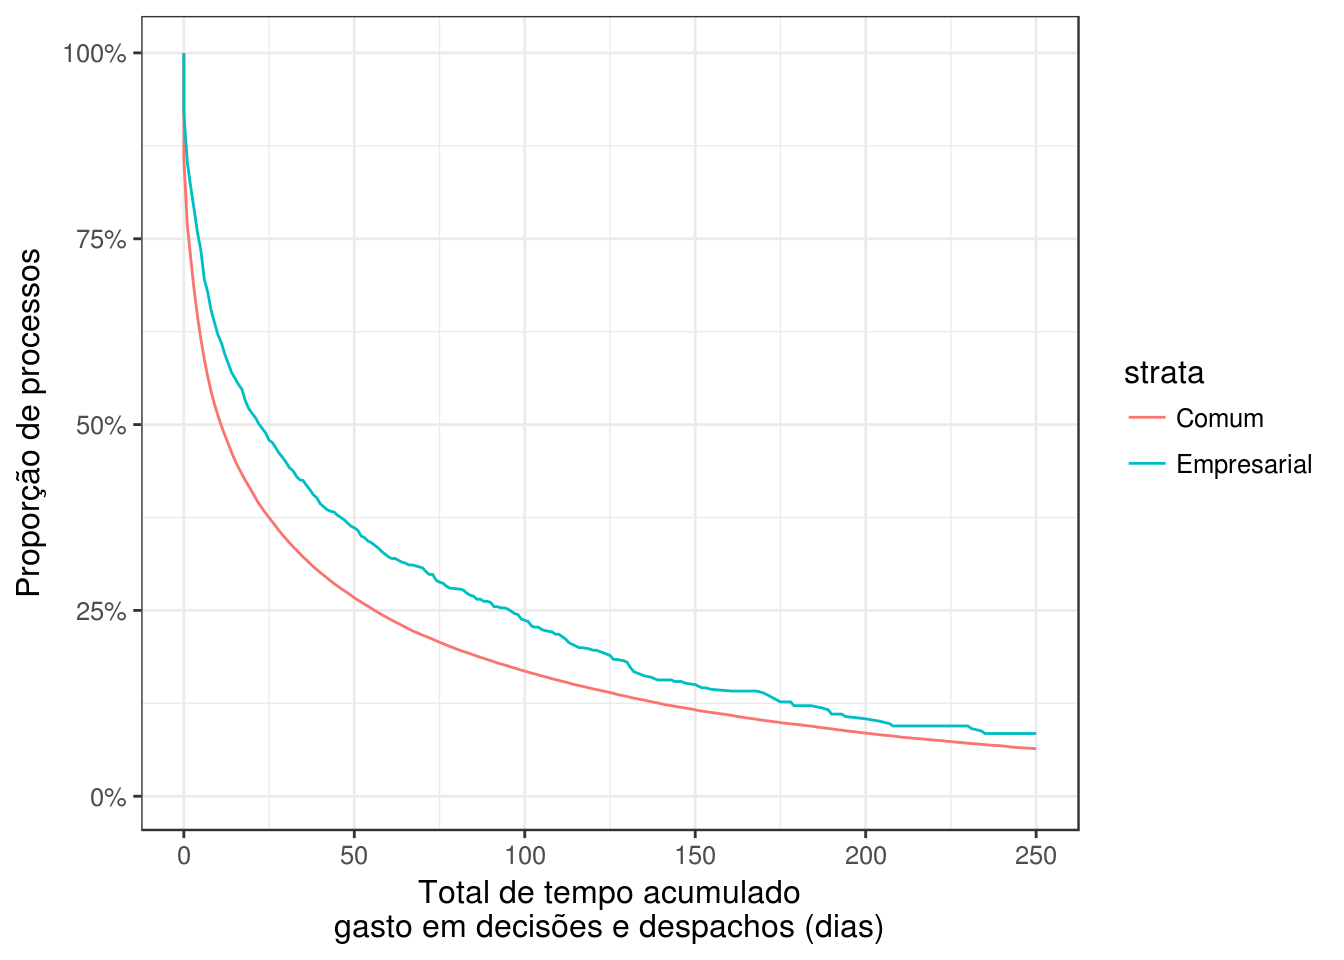
\includegraphics{tjspBook_files/figure-latex/sobrev-1.pdf}
\caption{\label{fig:sobrev}Curva de sobrevivência dos tempos acumulados
gastos em decisões e despachos (dias).}
\end{figure}

Essa observação mostra que a carga de trabalho associada a processos
empresariais é maior do que a carga associada a processos comuns.
Entretanto, a fim de calcular a taxa \(T_{E,C}\), precisamos de uma
medida-resumo da diferença entre as duas curvas. Um resumo natural para
curvas de sobrevivência é a quantidade de dias superada por exatamente
metade dos processos observados, que é a mediana do tempo total gasto em
decisões e despachos. Adotando esse critério, a comparação das duas
curvas sugere o valor de \(T_{E,C}\) fixado deve ser igual a 2.09.

\section{Foros regionais}\label{regionais}

A Secretaria de Planejamento do TJSP (SEPLAN), a pedido da Corregedoria
Geral, produziu um relatório analítico contendo levantamentos de dados
sobre processos empresariais nas varas da Comarca de São Paulo. Ao
contrário do presente estudo, que limita-se ao Foro Central Cível, esse
relatório estende suas considerações para os processos distribuídos no
Foros Regionais, e propõe uma metodologia de contagem de processos
similar a apresentada pela ABJ.

A partir de uma lista de assuntos elaborada junto à Corregedoria, a
SEPLAN apurou que aproximadamente 60\% dos processos empresariais
tramitam no Foro Central Cível. Assim, consideramos para os fins da
análise que \(p = 0.6\), mesmo que os dois relatórios divirjam com
relação a escolha de assuntos associados à processos de matéria
empresarial.

\chapter{Conclusão}\label{conclusao}

A partir dos valores estimados, concluímos que o número efetivo de
processos distribuídos por ano é

\[
N_e = \frac{N \times T_{E,C}}{p} = \frac{961 \times 2.09}{0.6} = 3349.
\]

Considerando apenas o critério de 1800 feitos por ano, o volume efetivo
anual de processos observado justifica a criação de pelo menos uma vara
empresarial. No entanto, considerando a sobra de mais de 1500 processos,
concluímos que a instalação de uma única vara pode sobrecarregar o
trabalho dos novos magistrados. Por isso, sugerimos, num cenário ideal,
a solução desse problema através da instalação de duas varas
especializadas, mas consideramos também que até mesmo a instalação de
uma única vara com dois juízes já seria satisfatória.

Por fim, ressaltamos que a instalação da(s) vara(s) precisa ser
acompanhada com métricas de produtividade adequadas. Para isso, será
necessário registrar o volume mensal de processos distribuído na(a)
vara(s), avaliando se a especialização reduz o tempo mediano dos
processos e a taxa de reforma de decisão.

\chapter{Apêndice}\label{apendice}

\begin{longtable}[t]{lll}
\caption{\label{tab:cnj}Tabela de assuntos empresariais, baseada na tabela de assuntos do CNJ e na resolução 623/2013 do TJSP.}\\
\toprule
assunto & Dispositivo Legal & Artigo\\
\midrule
Propriedade Intelectual / Indust... & Lei n? 9.609 de 19/02/1988, eLei... & \\
Desenho Industrial & Lei 9279/96 & arts 2?, II, 94 A 237\\
Marca & Lei 9279/96 & arts 2?, III, 122 a 216\\
Patente & Lei 9279/96 & arts 2?, I, 229 a 237\\
Anonima & Lei n? 10.406/02 (Codigo Civil) - & Arts 1088 a 1092\\
\addlinespace
Coligadas & Lei n? 10.406/02 (Codigo Civil) - & Arts 1097 a 1101\\
Comandita por Acoes & Lei n? 10.406/02 (Codigo Civil) - & Arts 1090 a 1092\\
Comandita Simples & Lei n? 10.406/02 (Codigo Civil) - & Arts 1045 a 1051\\
Conta de Participacao & Lei n? 10.406/02 (Codigo Civil) - & Arts 991 a 996\\
Cooperativa & Lei n? 10.406/02 (Codigo Civil) - & Arts 1093 a 1096\\
\addlinespace
Em comum / De fato & CCB & 986\\
Estrangeira & Lei n? 10.406/02 (Codigo Civil) - & Arts 1134 a 1141\\
Limitada & Lei n? 10.406/02 (Codigo Civil) - & Arts 1052 a 1087\\
Nome Coletivo & Lei n? 10.406/02 (Codigo Civil) - & Arts 1039 a 1044\\
Simples & Lei n? 10.406/02 (Codigo Civil) - & Arts 997 a 1038\\
\addlinespace
Alteracao de capital & Lei n? 10.406/02 (Codigo Civil) ... & Art: 1081 a 1084\\
Apuracao de haveres & Lei n? 10.406/02 & Art 1031\\
Cisao & Lei n? 10.406/02 (Codigo Civil) - & Art 1122\\
Coligacao & Lei n? 10.406/02 (Codigo Civil) - & Arts 1097 a 1122\\
Constituicao & Lei n? 10.406/02 (Codigo Civil) ... & Arts 997 a 1000\\
\addlinespace
Dissolucao & Lei n? 10.406/02 (Codigo Civil) ... & Arts 1033 a 1038\\
Fusao & Lei n? 10.406/02 (Codigo Civil) ... & Arts 1033 a 1038\\
Incorporacao & Lei n? 10.406/02 (Codigo Civil) - & Arts 1116 a 1118\\
Ingresso e Exclusao dos Socios n... & Lei n? 10.406/02 (Codigo Civil) - & Art 1057 e 1028 a 1032 e 1004\\
Liquidacao & Lei n? 10.406/02 (Codigo Civil) - & Arts 1102 a 1112\\
\addlinespace
Responsabilidade dos socios e ad... & Lei n? 10.406/02 (Codigo Civil) - & Art 1022 a 1027\\
Transferencia de cotas & Lei n? 10.406/02 (Codigo Civil) - & Art 997 e 999\\
Transformacao & Lei n? 10.406/02 (Codigo Civil) - & Arts 1113 a 1115\\
Agencie e Distribuicao & Lei n? 10.406/02 (Codigo Civil) - & arts 710 a 721;\\
Franquia & Lei Federal n? 8955/94; & art 2?\\
\addlinespace
Debentures & Lei Federal n? 6404/76, art. 72; & art 52\\
Assembleia & Lei n? 10.406/02 (Codigo Civil) ... & arts 59 e 60\\
Assembleia & Lei 10406/02 & Art 67\\
Administracao de heranca & Lei 10406/02 & 1791; 1797; 1991\\
Inventario e Partilha & Lei 10406/02, Lei 5869/73 e Lei ... & 1796 (CC), 983 (CPC) e 1o (Lei 6...\\
\addlinespace
Nulidade e Anulacao de Partilha ... & Lei 10406/02 e CPC & 2027 (CC); 1029 (CPC)\\
Sub-rogacao de Vinculo & Lei 10406/02 (Codigo Civil e Lei... & CC, art 1911, paragrafo unico; C...\\
Cometidos por Meio de Marca, Tit... & Lei 9.279/96 & Art 191\\
Contra as Marcas & Lei 9.279/96 & Art 189 a 190\\
Contra Indicacoes Geograficas e ... & Lei 9.279/96 & Arts 192 a 194\\
\addlinespace
Contra os Desenhos Industriais & Lei 9.279/96 & art 187 a 188\\
Contra Patente de Invencao & Lei 9.279/96 & art 183 a 186\\
De Concorrencia Desleal & Lei 9.279/96 & Art 195\\
Crimes Cometidos por Meio de Mar... & Lei 9.279/96 & Art 191\\
Crimes contra as Marcas & Lei 9.279/96 & Art 189 a 190\\
\addlinespace
Crimes contra Indicacoes Geeogra... & Lei 9.279/96 & Arts 192 a 194\\
Crimes contra os Desenhos Indust... & Lei 9.279/96 & art 187 a 188\\
Crimes contra Patente de Invencao & Lei 9.279/96 & art 183 a 186\\
Crimes de Concorrencia Desleal & Lei 9.279/96 & Art 195\\
\bottomrule
\end{longtable}

\end{document}
